\newpage

\section*{Ziel}
Im Folgenden soll das Zeitgesetz von gedämpften elektrischen Schwingungen untersucht und mit
der Theorie verglichen werden.
Zudem soll die Erscheinung einer Resonanz eines Schwingkreises 
durch eine erzwungende Schwingung analysiert werden.

\section{Theorie}
Ein RCL-Kreis besteht aus zwei Speicher Bausteinen. Einer Kapazität $C$ (Kondensator)
und einer Induktivität $L$ (Spule) sowie aus einem ohmschen Widerstand $R$.
Der Strom pendelt dabei zwischen den Speichern hin und her, während der Widerstand die 
elektrische Energie irreversibel in Joulsche Wärme umwandelt, und zu einer dämpfung der
Schwingung führt.

\begin{figure}
    \centering
    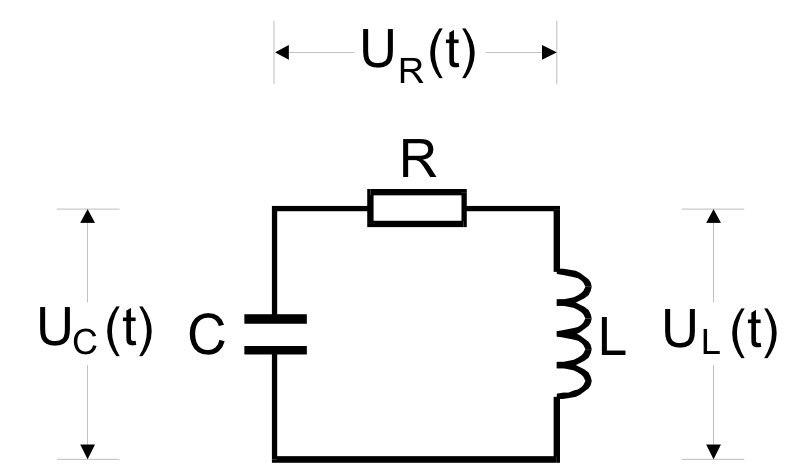
\includegraphics[width=0.4\textwidth]{bilder/schwing_allgemein.jpg}
    \label{fig:schwing_allgemein}
    \caption{Gedämpfte Schwingkreis mit Widerstand $R$,Kapazität $C$, Induktivität $L$ \cite[284]{Anleitung}}
\end{figure}

Über die 2. Kirchhoffsche Regel ergibt sich für die Spannung
\begin{equation}
    U_R(t)+U_C(t)+U_L(t)=0
\end{equation}
mit
\begin{align*}
    U_R(t)&=R \cdot I(t)\\
    U_C(t)&=\frac{Q(t)}{C}\\
    U_L(t)&=L\frac{dI}{dt}\\
    I(t)&=\frac{dQ}{dt}
\end{align*}
ergibt sich
\begin{equation}
    \frac{d^2I}{dt^2}+\frac{R}{L}\frac{dI}{dt}+\frac{1}{LC}I=0
\end{equation}
woraus das charakteristische Polynom folgt.
\begin{equation}
    k^2+\frac{R}{L}k+\frac{1}{LC}=0
\end{equation}
mit dem Ansatz $I(t)=Ae^{kt}$ ergibt sich mit der pq-Formel
\begin{equation}
    k=-\frac{R}{2L} \pm \sqrt{(\frac{R}{2L})^2-\frac{1}{LC}}                          %große Klammern einfügen 
\end{equation}
\label{eqn:k}
Der Schwingfall ergibt sich damit für die Bedingung, dass der Wurzelinhalt 
aus \eqref{eqn:k} negativ ist. Also
\begin{equation}
    \frac{R^2}{4L^2}<\frac{1}{LC}
\end{equation}
Das Folgerung ist ein oszillierender Strom
\begin{equation}
    I(t)=Ae^{-\frac{R}{2L}t}cos(\sqrt{\frac{1}{LC}-(\frac{1}{2L})^2}t)
\end{equation} 
Dabei ist der Faktor $\frac{R}{2L}$ für die einhüllende Form verantwortlich,
er beschreibt die Dämpfung der Schwingung wobei der ohmsch Widerstand $R$ als 
Dämpfungswiderstand bezeichnet wird.\\

Ist der Wurzelausdruck aus \eqref{eqn:k} $\sqrt{[...]}=0$
so spricht man vom aperiodischen Grenzfall, hierfür gilt die Bedingung
\begin{equation}
    \frac{R_{ap}^2}{4L}=\frac{1}{LC}
\end{equation}
hieraus ergibt sich für den Strom die Form
\begin{equation}
    I(t)=Ae^{-\frac{R}{2L}t}=Ae^{-\frac{t}{\sqrt{LC}}}
\end{equation}
Dabei konvergiert die Funktion am schnellsten gegen Null ohne eine Überschwingung.\\\\

Zur Untersuchung frequenzabhängiger Resonanz innerhalb des Schwingkreises durch
eine oszillierende Erregerspannung $\tilde{U}(w)$ mit einer Maximalamplitude $U_0$
wird die Kondensatorspannung $U_C$ in abhängigkeit der Frequenz $w$ gemessen.
Es gilt der Zusammenhang
\begin{equation}
    U_C(w)=\frac{U_0}{\sqrt{(1-LCw^2)^2+w^2R^2C^2}}
\end{equation}
Die Resonanzfrequenz $w_{res}$ ist dabei die Frequenz bei der das Verhältnis 
$\frac{U_C(w)}{U_0}$ ihren Maximum erreicht.
\begin{equation}
    w_{res}=\sqrt{\frac{1}{LC}-\frac{R^2}{2L^2}}
\end{equation}
\newpage
Die frequenzabhängige Phase zwischen $U_C(w)$ und $\tilde{U}(w)$ läst sich
dabei über den Vergleich des zeitlichen Abstandes $a$ der Nulldurchgänge 
mit der Länge $b$, der Schwingungsdauer bestimmen.
\begin{figure}
    \centering
    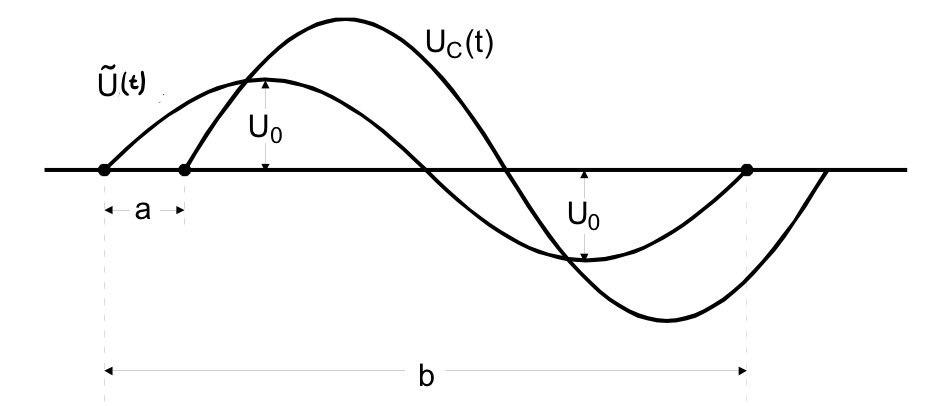
\includegraphics[width=0.65\textwidth]{bilder/phase.jpg}
    \caption{Methode zur Phasenbestimmung zwischen $U_C$ und $\tilde{U}$}
\end{figure}
somit gilt für die Phase $\phi$
\begin{equation}
    \phi = \frac{a}{b}\cdot 2\pi
\end{equation}


\label{sec:theorie}